\section{結果を描画する:net2g} \label{sec:quicklook}
%####################################################################################

SCAL-RMEモデルの出力ファイルは、
MPIプロセス毎に計算領域が分割されて、
別々のファイルとして出力される。
それぞれのファイルフォーマットは、
気候・予報(CF)メタデータ規約に対応したNetCDF4形式である
\footnote{gpviewがインストールされている場合、gpviewを使って作図することも出来る。
gpviewならばhistoryデータを変換することなく直接作図することができるため、クイックチェックに適している。}。
ここでは、1) プロセス毎に分割された{\netcdf}ファイルを
{\grads}で扱えるように1つのバイナリーファイルにまとめ、
2) 作図して結果の確認を行う。

\subsubsection{{\grads}バイナリーに変換}
%-----------------------------------------------------------------------------------
プロセスごとに分割された{\netcdf}形式のhistoryファイルから
{\grads}バイナリー変換するには、\verb|net2g|を使用する。
詳細な使用方法は \ref{sec:net2g}節を参照頂くこととして、
ここでは最低限の手続きのみ説明する。まず、net2gディレクトリへ移動する。
\begin{verbatim}
 $ cd ${Tutorial_DIR}/real/experiment/net2g
\end{verbatim}

\ref{sec:source_net2g}節でコンパイルしたバイナリーファイルに
リンクが貼られている。
\begin{verbatim}
 $ ln -s ../../../../util/netcdf2grads_h/net2g ./
\end{verbatim}
ここでは例として、2次元変数であるMSLP、PRECを、
3次元変数として850hPa,500h,200hPa面のU、Vを変換する.
2次元変数のための設定ファイルは\verb|net2g.2D.d01.conf|に、
3次元変数のための設定ファイルは\verb|net2g.3D.d01.conf|に用意している。

\verb|netcdf2grads_h|実行時のプロセス数は、
計算実行時に使用したプロセス数の約数である必要がある。
ここでは、計算に用いたのと同じ4プロセスを使用する。
現在、net2gでは2次元変数と3次元変数を同時に変換することはできないため、
それぞれに実行する。
\begin{verbatim}
 $ mpirun -n 4 ./net2g net2g.2D.d01.conf
 $ mpirun -n 4 ./net2g net2g.3D.d01.conf
\end{verbatim}
エラーメッセージがなく、下記のメッセージだけが標準出力へ表示されていれば正常に変換完了である。\\

\noindent {\gt
\fbox{
\begin{tabularx}{140mm}{l}
\verb|+++ MPI COMM: Corrective Finalize| \\
\end{tabularx}
}}\\

成功すれば、下記のファイルが作成される。
\begin{verbatim}
  MSLP_d01z-2d.ctl
  MSLP_d01z-2d.grd
  PREC_d01z-2d.ctl
  PREC_d01z-2d.grd
  U_d01z-3d.ctl
  U_d01z-3d.grd
  V_d01z-3d.ctl
  V_d01z-3d.grd
\end{verbatim}


\subsubsection{計算結果の確認}
%-----------------------------------------------------------------------------------
現在のバージョンの\verb|net2g|では、
SCALE-RMのXY格子座標で、ctlファイルを作成する。
今後、緯度経度座標で描画するためのctlファイルを
出力できるようにする予定であるが、
現バージョンは未対応のため、緯度経度座標で作図するためのctlを
\verb|${Tutorial_DIR}/real/data|ディレクトリに用意してある。
コピーしてい使用してほしい。
\begin{verbatim}
 $ cp ../../data/*_lcc.ctl ./
 $ ls
  MSLP_d01z-2d_lcc.ctl
  PREC_d01z-2d_lcc.ctl
  U_d01z-3d_lcc.ctl
  V_d01z-3d_lcc.ctl
\end{verbatim}

計算結果確認用の図を作成するためのスクリプト\verb|checkfig.gs|を使って作図する。
\begin{verbatim}
 $ cp ../../data/checkfig.gs ./
 $ grads -blc checkfig.gs
\end{verbatim}
成功すると、下記の図が作成される。
なお、GrADSのバージョンによって文法が異なるので、Warningが出る場合は、適宜変更する。
\begin{verbatim}
  real_mslp.png
  real_prec.png
  real_wind.png
\end{verbatim}
計算と変換が成功していれば、下記と同じ図が描画される。

\begin{figure}[h]
\begin{center}
  \includegraphics[width=0.55\hsize]{./figure/real_mslp.eps}\\
  \caption{計算開始から6時間後の海面更正気圧}
  \label{fig:real_mslp}
\end{center}
\begin{center}
  \includegraphics[width=0.55\hsize]{./figure/real_prec.eps}\\
  \caption{計算開始から6時間後の降水フラックス}
  \label{fig:real_prec}
\end{center}
\begin{center}
  \includegraphics[width=0.55\hsize]{./figure/real_wind.eps}\\
  \caption{計算開始から6時間後の500hPaの風速と風ベクトル}
  \label{fig:real_wind}
\end{center}
\end{figure}

\proofcomment{熱力学が変わったため、結果が異なるはずです。この図は、5.0.0リリース版で作りました。作り直しが必要と思います。}

